\section{Implementation}

We have implemented the system following best practices and leveraging popular tools and frameworks. The core system is in python. Python libraries MySQLdb, SQLAlchemy, psycopg2 are used to interact with the various data sources. Python library requests and BeautifulSoup are used in scraping citation data and properly parsing them. Flask framework is used for the service interface and Web GUI. Various JavaScript libraries such as highcharts are utilized in the web tier.

Publication and citation data retrieval is probably the foremost work so we detail the process in the following.

\subsection{Publication Data Acquisition}

\begin{figure}[htb]
  \centering
    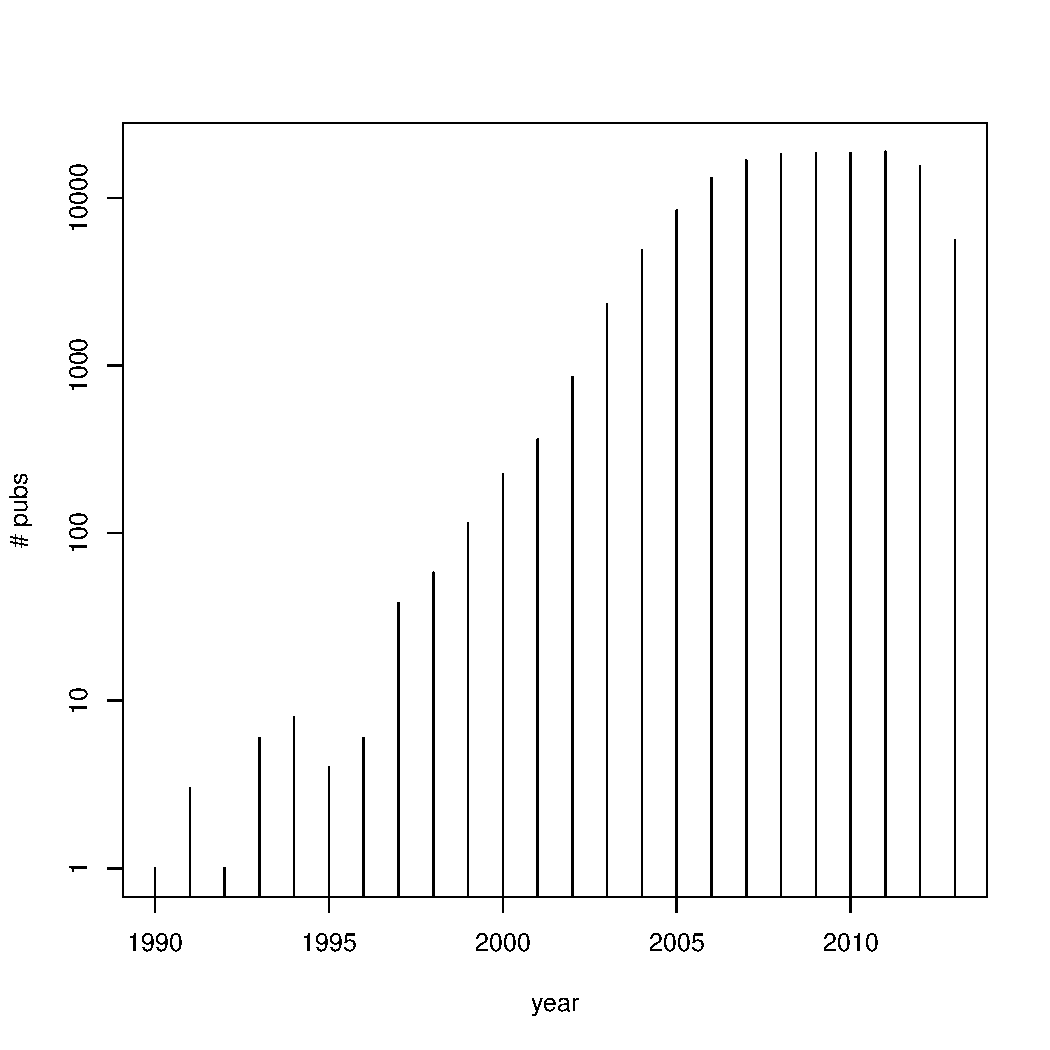
\includegraphics[width=1.0\columnwidth]{images/21_pubs_year_distribution.pdf}
  \caption{Publications by Year}\label{F:pubs-year-distribution}
\end{figure}

\begin{figure}[htb]
  \centering
    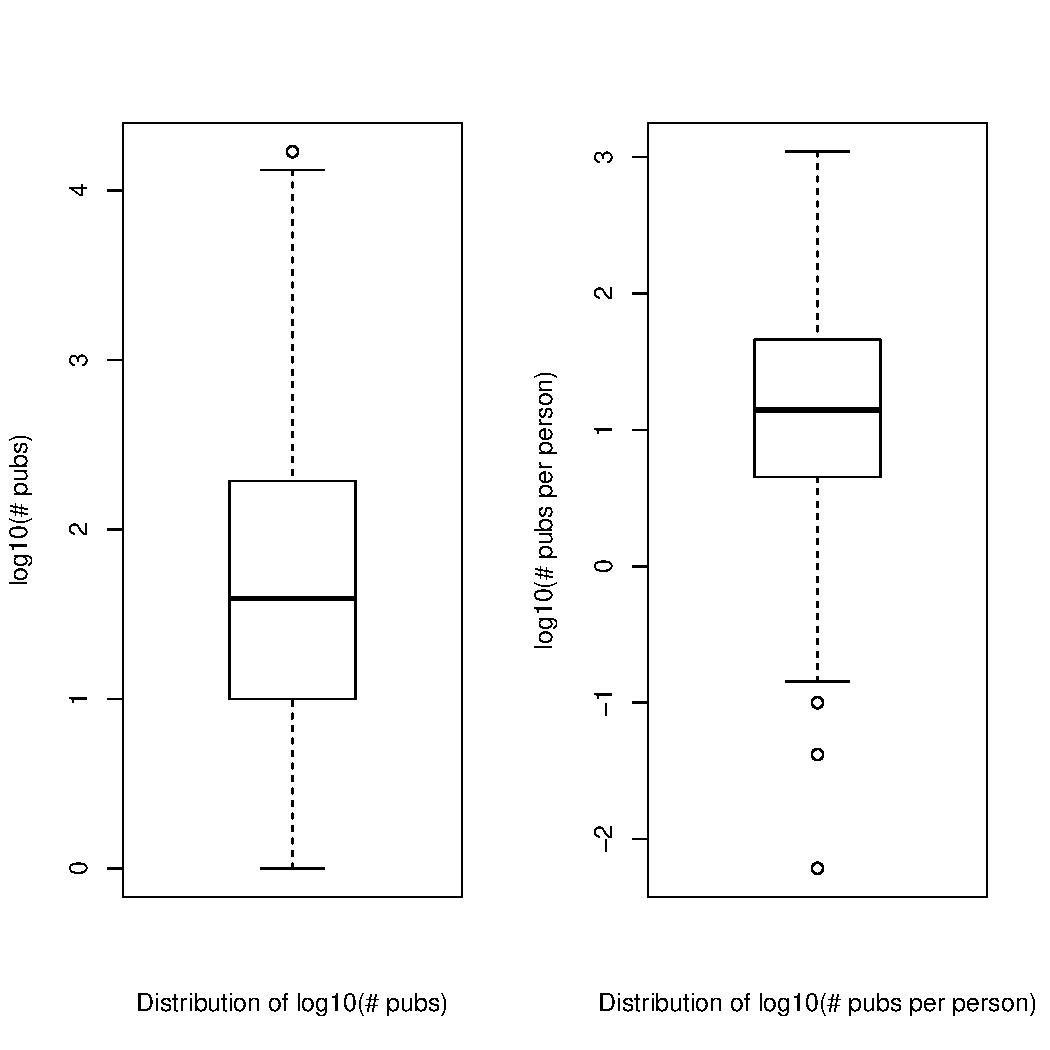
\includegraphics[width=1.0\columnwidth]{images/01_dist_npubs_proj.pdf}
  \caption{Distribution of number of publications}\label{F:dist-npubs-proj}
\end{figure}

We started the project by following the automated approach to obtain publication data. Publication citation data are available via subscribed resources such as ISI Web of Science \cite{www-isiwos} or open access such as Google Scholar \cite{www-googlescholar}, Microsoft Academic Search \cite{www-msas}, and Mendeley \cite{www-mendeley}, however they usually don't provide unlimited access.

Another approach which is probably more ideal is to get publication data from users. The user curated data tend to be more accurate comparing to automated mining, besides, there is another benefit that it gives extra information regarding a publication's association with the system, e.g., to which project it belongs. FutureGrid leveraged the drupal biblio module \cite{www-drupal-bib} with some customized design to support easy publication report and mass import via users or a staff member, and associated the publications with the related projects \cite{www-fgbiblio}. XSEDE now also provides a similar functionality via the portal \cite{www-xdportalpub}. nanoHUB citation analysis \cite{www-nanohubcite} as we have mentioned is also based on publication data submitted by users via a web form.

The framework itself supports pluggable data sources via mining databases and/or accessing 3rd party service APIs. We have experimented various data sources including Microsoft Academic Search, Google Scholar including user profile, and mining NSF award search data that are available upon request from NSF. The obtained data are then stored into the Mashup database which provides a common interface to other components in the system as well as collaborating systems like XDMOD.

In this study we focus only on two data sources - the user submitted data via XSEDE, and the NSF award search data for automated mining. The former source has user curated data with project affiliation information, thus it could give a measure on `direct' impact of XSEDE. However as it requires users' input, the former source currently has very limited data entries. The automated way obtains publication data for XSEDE users, which are not essentially direct output of using XSEDE resources, thus provides a measure on general or `indirect' impact of XSEDE. As a XSEDE user is affiliated with accounts/projects, and the projects are part of one or more FOS, we tag one publication as being related to the projects and FOSes based on these links. This is not most ideal but it provides a means to analyze the `indirect' impact on other levels in addition to users.

Based on the stated process, we were able to obtain over 142 thousand publication entries for over 20 thousand XSEDE users as of Jan 2014. Figure \ref{F:pubs-year-distribution} shows the yearly distribution of the publications. Figure \ref{F:dist-npubs-proj} shows distribution of number of publications by project (on the left) and by per user for each project.

\subsection{Citation Data Retrieval}

While for publication data user curated data might be more ideal, for citation data we have to go to the automated way for better accuracy and common grounds to compare. Google Scholar and ISI Web of Science provide such data, with some noticeable limitations. E.g., Google Scholar does not provide an API, nor it allows unlimited access within a bounded time period from one request source. ISI data does not impose a rate limiting while you have subscribed access, however it does not provide easy access API either. So one has to submit query via the web UI and then parse the data from the tabulated results list.

We have explored both approaches for a subset of the publication data, and did a comparison of the results. While similar comparison has been attempted \cite{yang2006citation} in a very small sample size - 2 people and about 100 publications, our study has included 33861 publications and 1462 users.

\begin{figure}[htb]
  \centering
    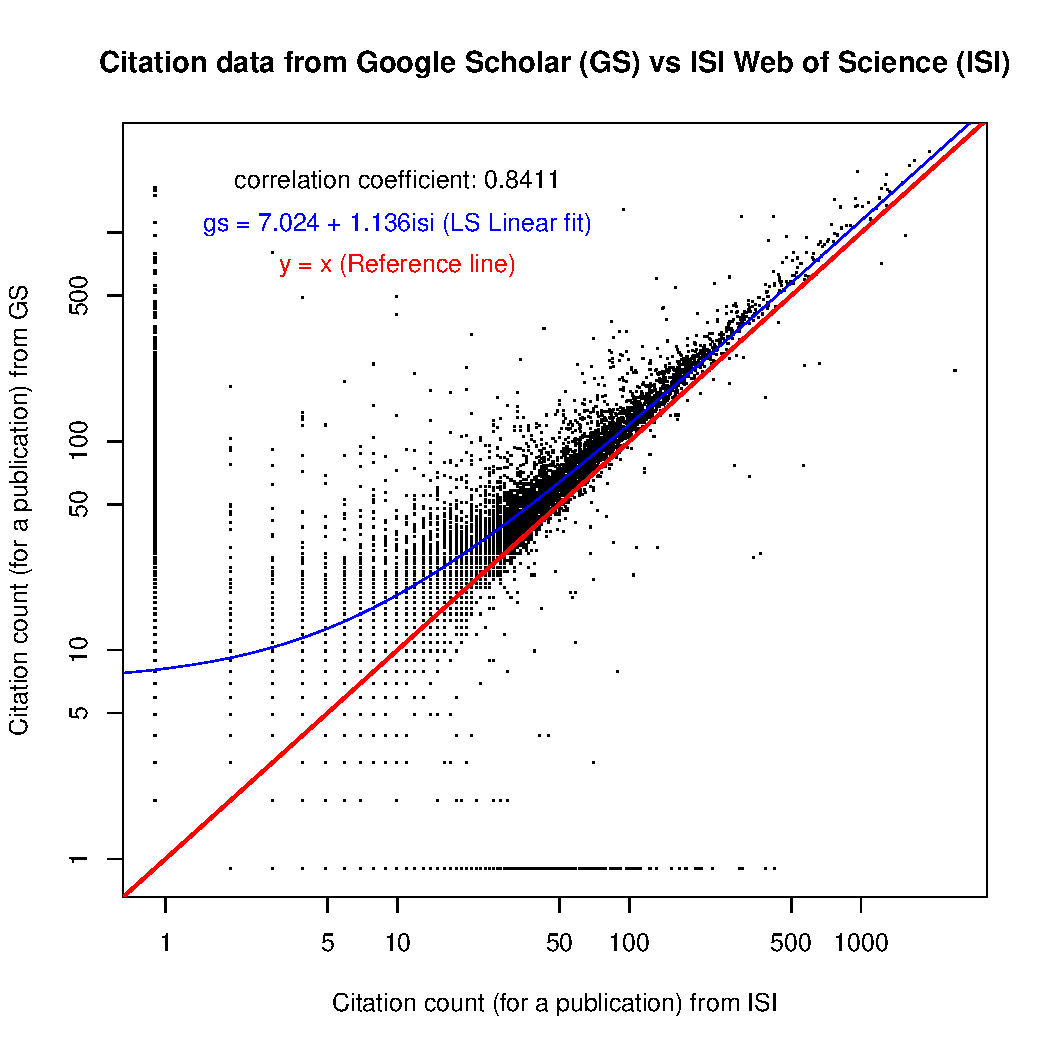
\includegraphics[width=1.0\columnwidth]{images/11_gs_vs_isi_cites.pdf}
  \caption{Citations (GS vs ISI)}\label{F:gs-vs-isi-cites}
\end{figure}

\begin{figure}[htb]
  \centering
    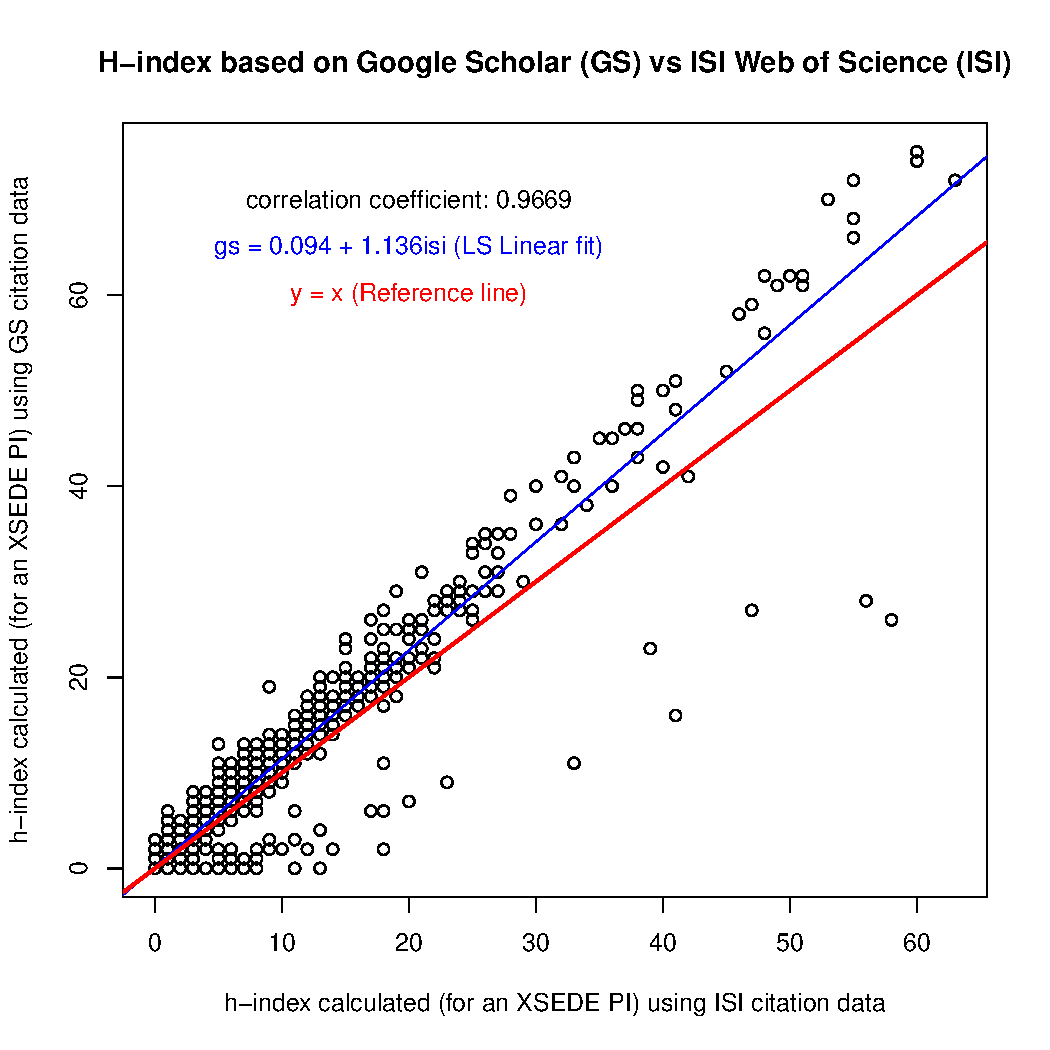
\includegraphics[width=1.0\columnwidth]{images/11_gs_vs_isi_hindex.pdf}
  \caption{H-index (GS vs ISI)}\label{F:gs-vs-isi-hindex}
\end{figure}

Figure \ref{F:gs-vs-isi-cites} shows the citation data from Google Scholar vs ISI Web of Science. Out of the 33861 data points, 20793 of them (61.4\%) have larger value in GS, 10315 (30.5\%) are the same, while 2753 (8.1\%) have larger value in ISI. 5287 (15.6\%) publications have zero citation found in ISI but non-zero in GS, 1253 (3.7\%) pubs have zero citaion in GS but non-zero in ISI. In general Google Scholar tends to have higher citation number.

Figure \ref{F:gs-vs-isi-hindex} shows that H-index obtained from Google Scholar data vs ISI data. Out of the 1462 data points, 663 of them (45.3\%) have larger value in GS, 677 (46.3\%) are the same, while 122 (8.3\%) have larger value in ISI.
52 (3.6\%) PIs have zero H-index computed from ISI data but non-zero from GS, 39 (2.7\%) for the reverse side. In general h-index calculated from Google Scholar data tends to be a bit higher.

In either case a high positive correlation is observed. The Pearson correlation coefficient are 0.84 and 0.97 respectively. The very strong correlation of the h-index values are mostly due to the fact that one of the two factors determining the h-index, the number of publications, stay the same for a perticular user.

Based on the study, while we don't have complete citation data from Google Scholar due to access restriction, we were able to use the ISI citation data to get very similar measures for most of the data especially for the h-index metric. Thus the following analyses are using the ISI citation data to further derive other metrics.
